\documentclass[10pt,a4paper,onepage,DIV12]{scrartcl}
% \areaset{210mm}{297mm}
\usepackage[T1]{fontenc}        %k.A.
\usepackage[latin1]{inputenc} %k.A.
%\usepackage{ngerman}   %Deutsch
\usepackage{amssymb,amsmath,amsthm}     %Mathe
\usepackage[pdftex]{graphicx} %Bilder
% \usepackage[german]{babel}
\usepackage[usenames,dvipsnames,pdftex]{color}
\usepackage[english]{babel}
\usepackage[font=small,labelfont=bf]{caption}
%\usepackage{bibgerm}
%\usepackage{subfig}
%\usepackage[subfigure]{tocloft}
\usepackage[colorlinks=true]{hyperref}
\setlength{\headheight}{15pt}
\usepackage{fancyhdr}
\usepackage{listings}
\usepackage{svn-multi}
\svnidlong
{$HeadURL$}
{$LastChangedDate$}
{$LastChangedRevision$}
{$LastChangedBy$}
\usepackage{url}



\usepackage{multicol}
\lstset{language=Matlab
, basicstyle=\ttfamily\scriptsize\bfseries
, keywordstyle=\color{Blue}\pmb
, breaklines=true
, commentstyle=\color{OliveGreen} 
, 
}
\lstset{numbers=left, stepnumber=2, numberstyle=\tiny, numbersep=5pt
%, frame=tb
}

\pagestyle{fancy}
\fancyhf{}
\lhead[\thepage]{\texttt{\svnkw{HeadURL}} -- Rev. \svnrev}
\rhead[\leftmark]{\thepage}

\title{Correlative Microscopy - Algorithm overview}
\author{Martin Schorb, \href{mailto:martin.schorb@embl.de}{martin.schorb@embl.de}}
\publishers{\small{\vspace{2mm} corresponds to revision \svnrev\; commited at \svndate}\\\small{ of \texttt{martin\_correlate.m} at \url{\svnkw{HeadURL}}}
}

\setlength{\columnsep}{10pt}

\begin{document}
 \maketitle
\section{Introduction}
This document describes the usage of the algorithms designed for correlation of fluorescence microscopy images to their corresponing EM image. 

The correlation procedure, as described in Kukulski et al.,... , consists of two major coordinate transformations. The first one uses fluorescent microspheres to calculate the mapping of a single point fluorescent signal onto an electron microscopy image of low resolution ($4-10 $k$\times$). The obtained coordinates can then be transformed further using a different fiducial system (in this case the gold beads used for tomogram reconstruction) to a high magnification image.

This document provides a step by step manual in how to use the algorithms, their parameters and outputs and shows the corresponding code snippets to give an idea of the points at which certain things happen while running the script.
\section{Installation and requirements}

\subsection{System and software requirements}A MATLAB\textsuperscript{\textregistered} 
installation version 7.4.0 onwards including the Image Processing Toolbox is required for succesfully running the scripts. This should be independent on the type of operating system used. However the function was so far only successfully tested on Linux environments. 
\\

In order to access the newest version of the scripts, a subversion (SVN\footnote{See \url{http://www.structures-it.embl.de/services/online/vcs},\; \url{http://en.wikipedia.org/wiki/Subversion}}) client is needed. In case you don't have access to a software capable of checking out subversion repositories, you can simply download all files individually from the webserver (\url{https://svn.structures/repo/schorb:Corr}).

\subsection{Obtaining the newest version of the correlation algorithms}

The main scripts as well as all supporting underlying algorithms and this documentation are stored in a central subversion repository which is accessible from within the EMBL network.
\subsubsection*{First installation}
To checkout the most recent version of algorithms and documentation files for the first time, create a directory where you want to store these files. Add this directory including all subdirectories to the MATLAB path by adding the following line to MATLAB's \texttt{startup.m} script, that is usually located in a MATLAB related folder within your home directory (\texttt{$\sim$/.matlab/startup.m} for Linux or Macintosh systems).
\begin{verbatim}
 addpath (genpath('/path/to/your/directory'),'-begin')
\end{verbatim}
Then checkout the files to this directory using your subversion client. The Unix Terminal command will be this:
\begin{verbatim}
 svn checkout https://svn.structures/repo/schorb:Corr /your/directory/
\end{verbatim}
You should see a result like this:
\begin{verbatim}

A    Corr/martin_correlate.m
A    Corr/martin_chromaticshift_drift2.m
...
A    Corr/john_manualregister_LMtoHMtomo3.m
Checked out revision 26.

\end{verbatim}

Now you have a local working copy of the most recent versions of the correlation files.

\subsubsection*{Updating your existing scripts}

To have your scripts and documentation files always up to date according to the current revision, update them from the repository by simply executing
\begin{verbatim}
 svn up
\end{verbatim}
 in the directory in which you put the scripts. 

\subsubsection*{Editing the scripts}
You can manipulate and edit your local working copy of the scripts (activate or remove sub-pixel fitting, shift correction etc.). However these changes will be reverted while updating to a newer revision. 

Also note that there will be some hidden files and directories (\texttt{.svn} etc.) written while checking out. These contain important information needed by subversion and should not be modified or deleted.

\subsubsection*{Initialization}

You can adjust key parameters of the correlation scrips by modifying the initialization script. When checking out the repository a file called \texttt{corr\_init\_orig.m} will appear. You can simply rename this filie to \texttt{corr\_init.m} and change the parameters and paths according to your needs. This file will then stay in your local scripts directory and will not be overritten.

 It might occur that in future revisions additional parameters will be added to this script, so in case you run into an error message stating this, just update your local \texttt{corr\_init.m} with the changes you find in the downloaded and most up-to-date \texttt{corr\_init\_orig.m}.


\section{Correlation from LightMicroscopy to LowMag EM image}

Correlation from the original fluorescence image to an appropriate EM image containing indentifiable fiducial markers is performed using the script \texttt{martin\_correlate}.

\subsection{Executing the script}
To execute the script and start the correlation simply run \begin{verbatim}
 martin_correlate(fmf,emf,gmf,rmf,outfileroot)
\end{verbatim}
 in the MATLAB command line.
 \lstinputlisting[linerange={1-8}]{../martin_correlate.m}
It requires the following input parameters:
\begin{enumerate}
 \item\texttt{fmf} -- path to FM image file containing fiducial information (1344$\times$1024 pixel, 8 or 16bit tiff-file)
 \item\texttt{emf} -- path to EM image file containing visible fiducials (2048$\times$2048 pixel, 8 or 16bit tiff-file)
 \item\texttt{gmf} -- path to FM image file containing point of interest in first channel -- considered to be GFP (same dimensions and format as fmf)
 \item\texttt{rmf} -- path to FM image file containing point of interest in second channel -- considered to be RFP (same dimensions and format as fmf)
 \item\texttt{outfileroot} -- directory and name base for generating output files.
\end{enumerate}

\subsection{Output and generated files}
The following files are generated by the correlation script during runtime. The name base is referred to as \texttt{BASE}. An appended \texttt{XFP} refers to the fluorescent channel chosen for correlation. The selected correlation that was used is denoted by either the transform number or \texttt{all} in case the transformation based on all beads was chosen (\texttt{\#}). 
\begin{itemize}
 \item \texttt{BASE\_picked1.txt} -- Plain text file containing the coordinates of fiducial pairs after subpixel fitting. \lstinputlisting[linerange={235-240}]{../martin_correlate.m}

\item \texttt{BASE.pickspots1.mat} -- Fiducial pair coordinates, input parameters, selected fluorescent channel and clicked fluorescence spot -- MATLAB format.\lstinputlisting[linerange={242-243}]{../martin_correlate.m}

 \item \texttt{BASE\_XFP\_fluoshift.shiftcoos.mat} -- Coordinates from bleed-through fiducials to determine shift in between the acquisition of images.(within \texttt{martin\_chromaticshift\_drift2} sub-script)
\lstinputlisting[linerange={41-41}]{../martin_chromaticshift_drift2.m}


\item \texttt{BASE\_XFP\_\#\_pred.tif} -- Overlay image showing the predicted and actual positions of the fiducials in EM coordinates. (size of EM-image, 16bit tiff-file)
\item \texttt{BASE\_XFP\_\#\_prediction.tif} -- Circle marking the position of the transformed coordinate of the spot of interest. (all images with same properties)
\item \texttt{BASE\_XFP\_\#\_pred\_overlay.tif} -- Overlay of the prediction circle and EM image
\item \texttt{BASE\_XFP\_\#\_fm.tif} -- Transformed fluorescent fiducial image 
\item \texttt{BASE\_XFP\_\#\_em.tif} -- electron microscopy image 
\item \texttt{BASE\_XFP\_\#\_gm.tif} -- Transformed image of first fluorescence channel (GFP)
\item \texttt{BASE\_XFP\_\#\_rm.tif} -- Transformed image of second fluorescence channel (RFP)
\item \texttt{BASE\_XFP\_\#\_tfmed.tif} -- Transformed fluorescence fiducial coordinates
\item \texttt{BASE\_XFP\_\#\_pickedem.tif} -- Picked EM coordinates

\item \texttt{BASE\_XFP\_\#\_transform.log} -- Plain text file containing the source files used for correlation, the transformed spot coordinates and various information about the used transformation
\end{itemize}

\subsection{User interaction and key procedures}
\subsubsection{Fiducial selection}
\label{sec:fiducials}
Fiducial pairs are selected in both LM and EM image using the \texttt{cpselect} tool. When an already existing coordinate file is opened, these are displayed. (Fig.\,\ref{fig:cpsel_fid1}) To continue, close the window.

\begin{figure}
 \centering
 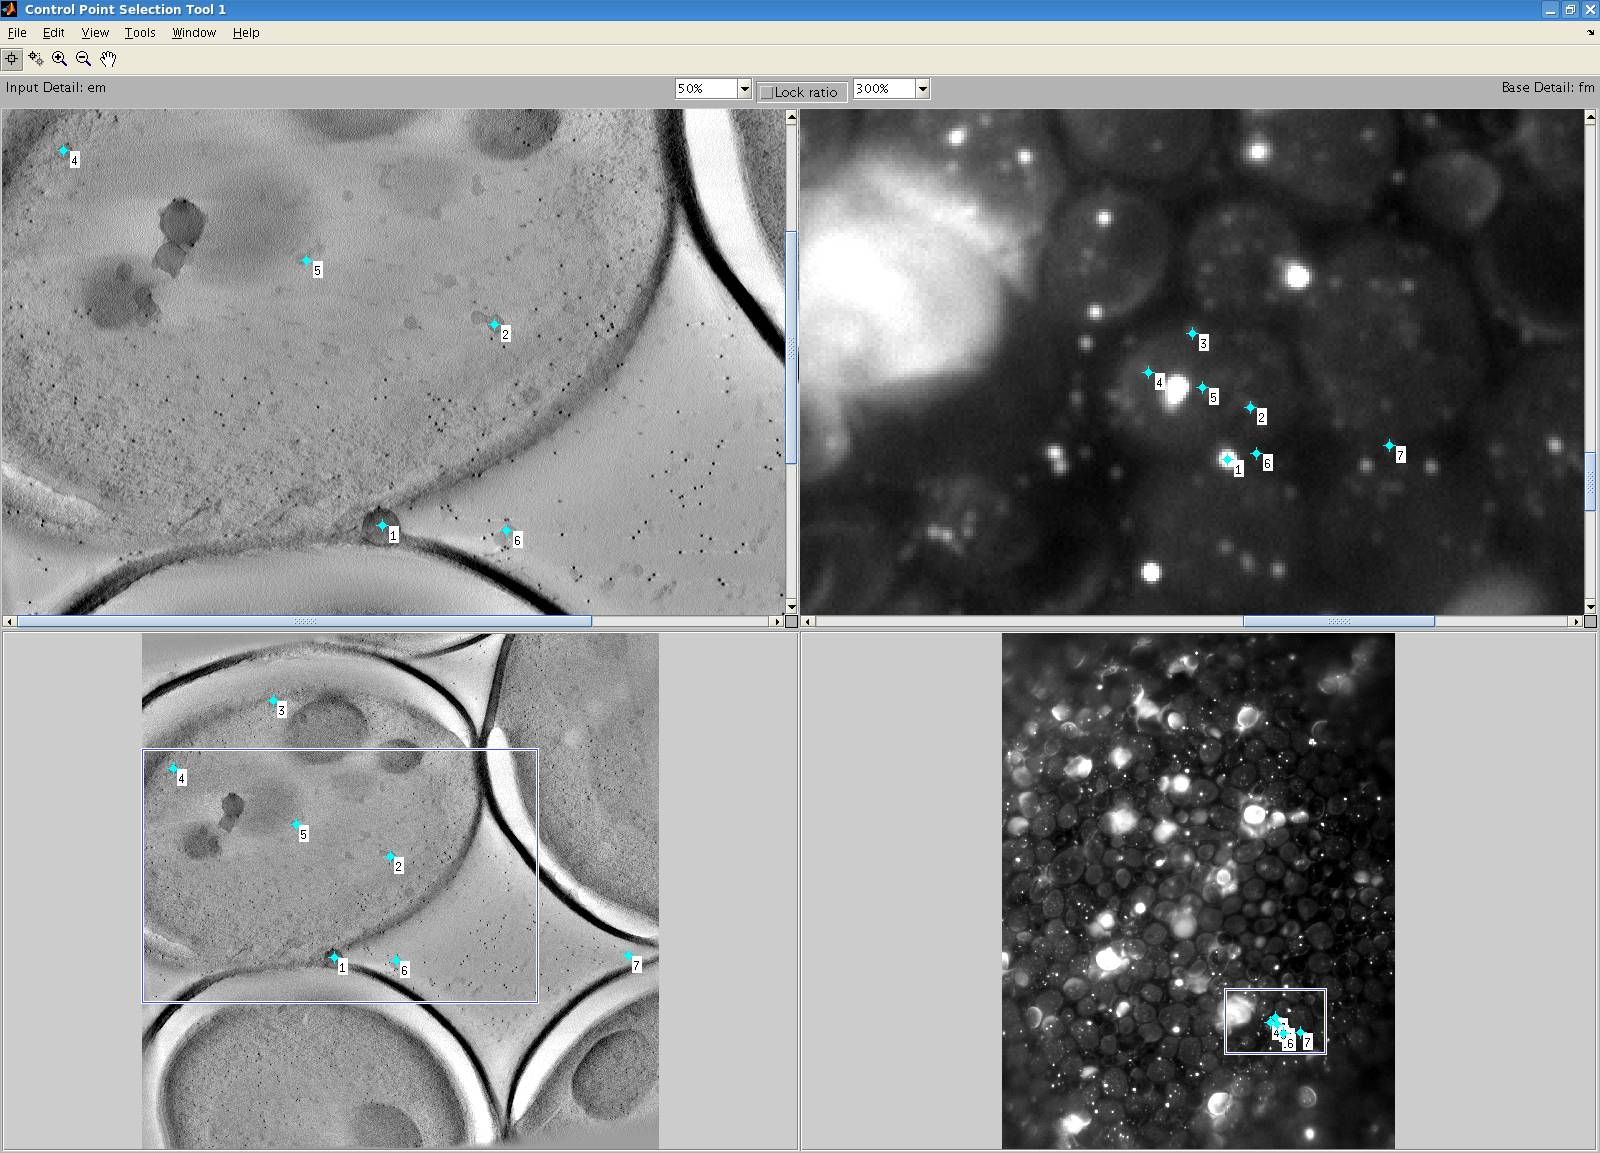
\includegraphics[width=.78\textwidth]{images/cpsel_fid1.jpg}
 % cpsel_fid1.png: 1600x1153 pixel, 72dpi, 56.44x40.68 cm, bb=0 0 1600 1153
 \caption{\texttt{cpselect} -- graphical interface for picking and checking fiducial positions}
 \label{fig:cpsel_fid1}
\end{figure}

\subsubsection{Fiducial sub-pixel fitting and display}
Fiducial positions in the light microscopy image are fitted with sub-pixel accuracy using a center of mass detection after high-pass filtering.
The fitted positions are presented again using a \texttt{cpselect} dialog. (Fig.\,\ref{fig:cpsel_fid1}) To continue, close the window.

 \lstinputlisting[linerange={157-157,205-206}]{../martin_correlate.m}

\subsubsection{Selection of fluorescence channel}
A popup window will ask you to determine the fluorescence channel in which your signal of interest is imaged.(Fig.\,\ref{fig:fluorsel})

\begin{figure}
 \centering
 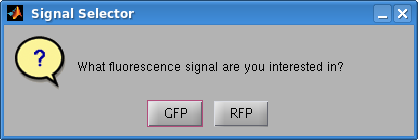
\includegraphics[width=.38\textwidth]{images/fluorsel.png}
 % fluorsel.png: 418x140 pixel, 72dpi, 14.75x4.94 cm, bb=0 0 418 140
\caption{graphical interface for selecting the fluorescence channel}
 \label{fig:fluorsel}
\end{figure}

\subsubsection{Picking the fluorescent spot of interest}
In the folowing \texttt{cpselect} dialog, the selected fluorescence image is shown on the right, the positions indicating the fiducial markers. Click once in the right image to determine the position of the spot of interest AND once in the left image just anywhere. This click in the left image will have no effect on the correlation. \texttt{cpselect} otherwise would just not export the clicked coordinates. In case you forget to click in the left image, a reminder will be shown and you have the chance to click again.
\begin{figure}
 \centering
 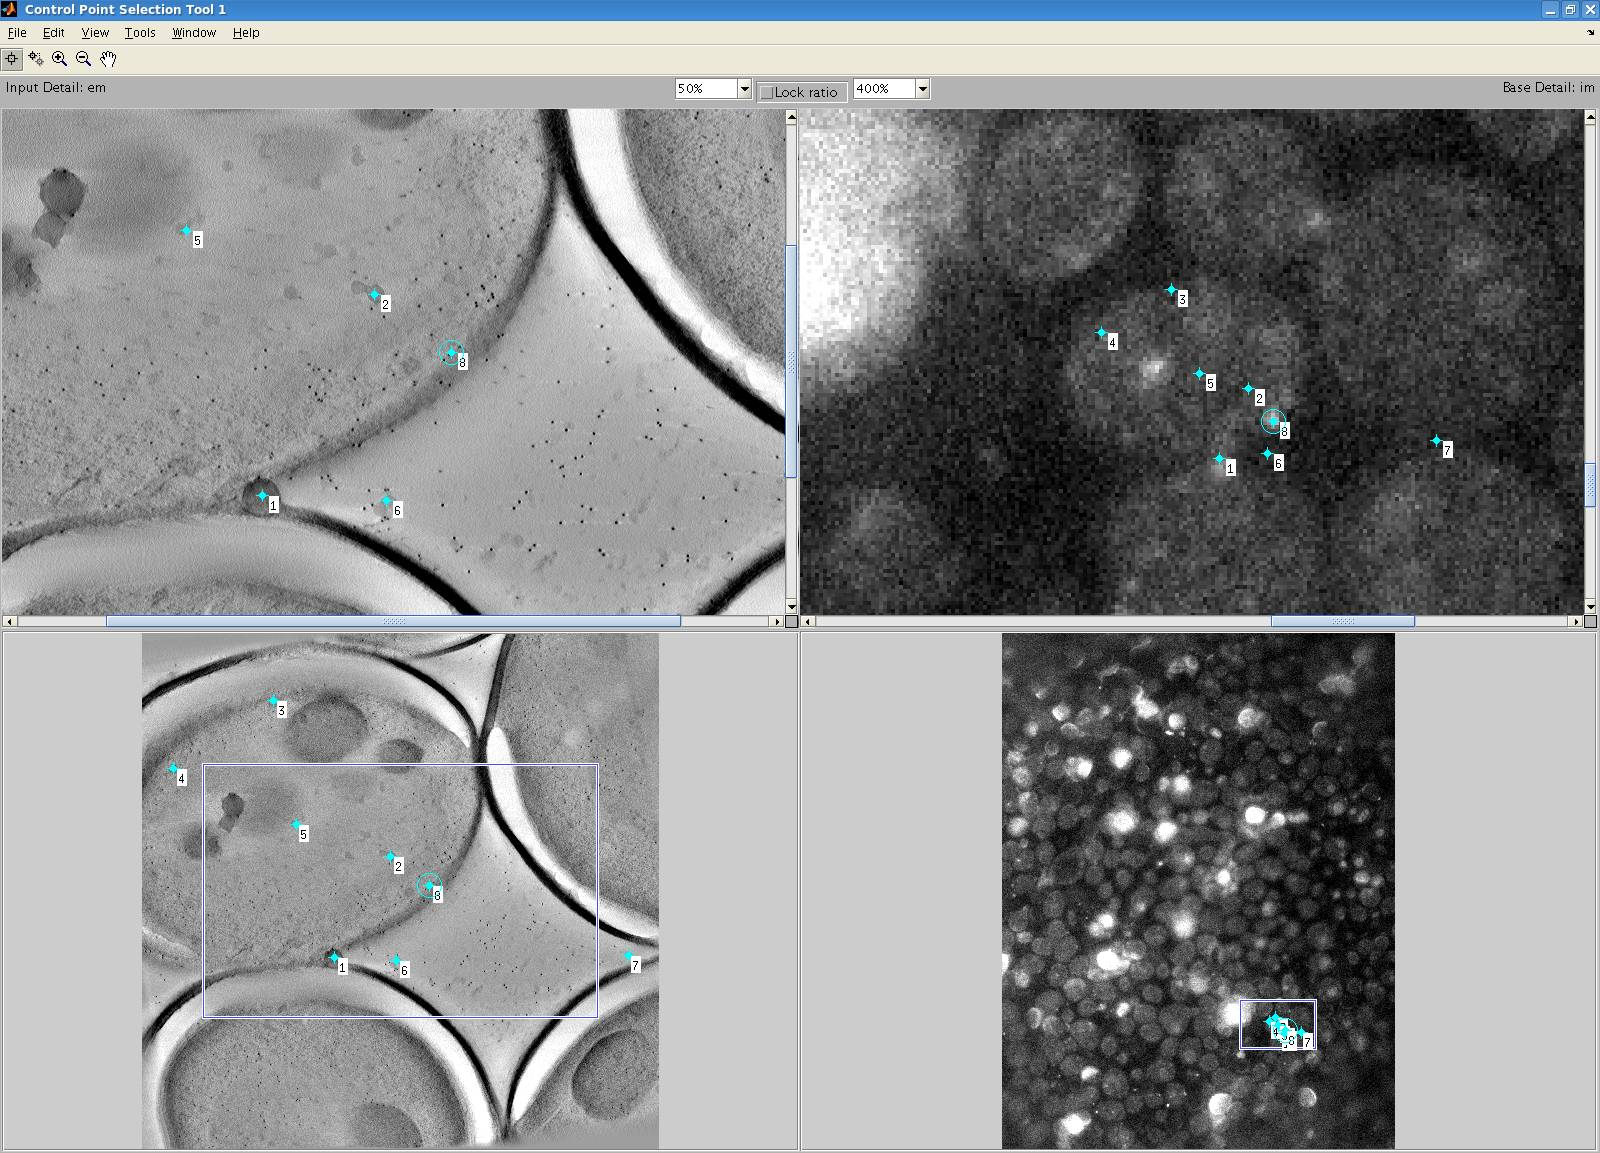
\includegraphics[width=.78\textwidth]{images/cpsel_fluor1.jpg}
 % cpsel_fluor1.png: 1600x1153 pixel, 72dpi, 56.44x40.68 cm, bb=0 0 1600 1153
 \caption{Selection of the fluorescent spot of interest -- marked spots \#8. The selected fluorescence channel image is shown on the right, the left click can be arbitrary.}
 \label{fig:cpsel_fluor1}
\end{figure}

\subsubsection{Sub-pixel fitting of the fluorescent spot of interest}
\begin{figure}
 \centering
 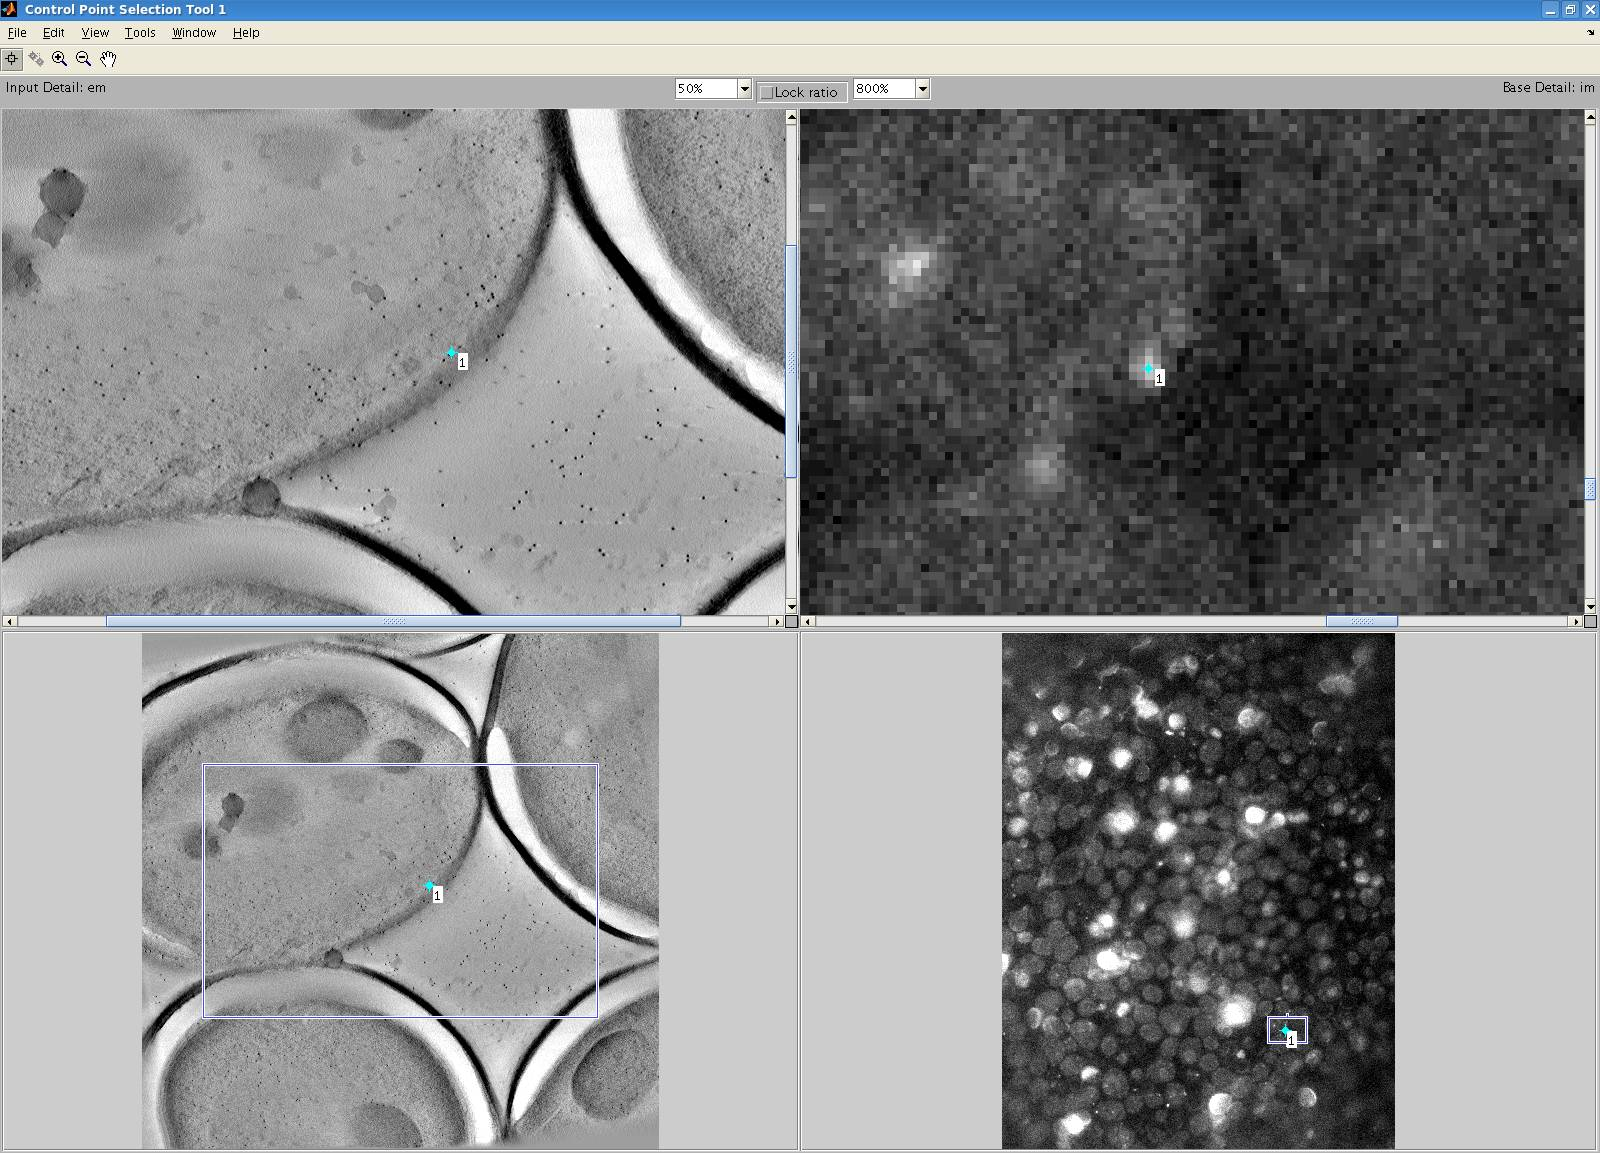
\includegraphics[width=.78\textwidth]{images/cpsel_fluor2.jpg}
 % cpsel_fluor2.png: 1600x1153 pixel, 72dpi, 56.44x40.68 cm, bb=0 0 1600 1153
 \caption{Positioning of the spot of interest after sub-pixel fitting}
 \label{fig:cpsel_fluor2}
\end{figure}
\end{document}